\documentclass[a4paper]{book}
\usepackage{a4wide}
\usepackage{makeidx}
\usepackage{graphicx}
\usepackage{multicol}
\usepackage{float}
\usepackage{listings}
\usepackage{color}
\usepackage{textcomp}
\usepackage{alltt}
\usepackage{times}
\usepackage{ifpdf}
\ifpdf
\usepackage[pdftex,
            pagebackref=true,
            colorlinks=true,
            linkcolor=blue,
            unicode
           ]{hyperref}
\else
\usepackage[ps2pdf,
            pagebackref=true,
            colorlinks=true,
            linkcolor=blue,
            unicode
           ]{hyperref}
\usepackage{pspicture}
\fi
\usepackage[utf8]{inputenc}
\usepackage{doxygen}
\lstset{language=C++,inputencoding=utf8,basicstyle=\footnotesize,breaklines=true,breakatwhitespace=true,tabsize=8,numbers=left }
\makeindex
\setcounter{tocdepth}{3}
\renewcommand{\footrulewidth}{0.4pt}
\begin{document}
\hypersetup{pageanchor=false}
\begin{titlepage}
\vspace*{7cm}
\begin{center}
{\Large grep \\[1ex]\large 1.0.0 }\\
\vspace*{1cm}
{\large Generated by Doxygen 1.7.1}\\
\vspace*{0.5cm}
{\small Fri Mar 18 2011 21:53:40}\\
\end{center}
\end{titlepage}
\clearemptydoublepage
\pagenumbering{roman}
\tableofcontents
\clearemptydoublepage
\pagenumbering{arabic}
\hypersetup{pageanchor=true}
\chapter{Data Structure Index}
\section{Data Structures}
Here are the data structures with brief descriptions:\begin{DoxyCompactList}
\item\contentsline{section}{\hyperlink{structparameter}{parameter} (Process parameter; )}{\pageref{structparameter}}{}
\end{DoxyCompactList}

\chapter{File Index}
\section{File List}
Here is a list of all files with brief descriptions:\begin{DoxyCompactList}
\item\contentsline{section}{\hyperlink{grep_8c}{grep.c} }{\pageref{grep_8c}}{}
\end{DoxyCompactList}

\chapter{Data Structure Documentation}
\hypertarget{structparameter}{
\section{parameter Struct Reference}
\label{structparameter}\index{parameter@{parameter}}
}


Process parameter;.  


\subsection*{Data Fields}
\begin{DoxyCompactItemize}
\item 
char \hyperlink{structparameter_a1ae211b923c0ca2de98c2a6b3ec4c6b1}{version}
\item 
char \hyperlink{structparameter_a1381e4a8fe53b36d133973f26e08cef4}{help\_\-info}
\item 
char \hyperlink{structparameter_a021dce247495584ddd423f072f04672c}{pattern}
\item 
char \hyperlink{structparameter_a4ecb9d8632a7871799de459d57e099ec}{file}
\item 
char \hyperlink{structparameter_a454fa9de3ca009e3082488412cd184d4}{option}
\item 
char \hyperlink{structparameter_a55fa74161839e8f2e73198c67ad074d7}{usage}
\item 
char \hyperlink{structparameter_a5d392da4ac3b837edcd0ea423f63ce60}{directory}
\item 
char $\ast$ \hyperlink{structparameter_a63ee2b43ba6b35b7de16d6d9da0b97e9}{pattern\_\-info} \mbox{[}10\mbox{]}
\item 
char $\ast$ \hyperlink{structparameter_ab8fcad04e42add1edf49b16b68b2585b}{file\_\-info} \mbox{[}10\mbox{]}
\item 
char $\ast$ \hyperlink{structparameter_adc4158a7ebdb2434c6fd85cc1110c226}{directory\_\-info} \mbox{[}10\mbox{]}
\end{DoxyCompactItemize}


\subsection{Detailed Description}
Process parameter;. 

\subsection{Field Documentation}
\hypertarget{structparameter_a5d392da4ac3b837edcd0ea423f63ce60}{
\index{parameter@{parameter}!directory@{directory}}
\index{directory@{directory}!parameter@{parameter}}
\subsubsection[{directory}]{\setlength{\rightskip}{0pt plus 5cm}char {\bf directory}}}
\label{structparameter_a5d392da4ac3b837edcd0ea423f63ce60}
\hypertarget{structparameter_adc4158a7ebdb2434c6fd85cc1110c226}{
\index{parameter@{parameter}!directory\_\-info@{directory\_\-info}}
\index{directory\_\-info@{directory\_\-info}!parameter@{parameter}}
\subsubsection[{directory\_\-info}]{\setlength{\rightskip}{0pt plus 5cm}char$\ast$ {\bf directory\_\-info}\mbox{[}10\mbox{]}}}
\label{structparameter_adc4158a7ebdb2434c6fd85cc1110c226}
\hypertarget{structparameter_a4ecb9d8632a7871799de459d57e099ec}{
\index{parameter@{parameter}!file@{file}}
\index{file@{file}!parameter@{parameter}}
\subsubsection[{file}]{\setlength{\rightskip}{0pt plus 5cm}char {\bf file}}}
\label{structparameter_a4ecb9d8632a7871799de459d57e099ec}
\hypertarget{structparameter_ab8fcad04e42add1edf49b16b68b2585b}{
\index{parameter@{parameter}!file\_\-info@{file\_\-info}}
\index{file\_\-info@{file\_\-info}!parameter@{parameter}}
\subsubsection[{file\_\-info}]{\setlength{\rightskip}{0pt plus 5cm}char$\ast$ {\bf file\_\-info}\mbox{[}10\mbox{]}}}
\label{structparameter_ab8fcad04e42add1edf49b16b68b2585b}
\hypertarget{structparameter_a1381e4a8fe53b36d133973f26e08cef4}{
\index{parameter@{parameter}!help\_\-info@{help\_\-info}}
\index{help\_\-info@{help\_\-info}!parameter@{parameter}}
\subsubsection[{help\_\-info}]{\setlength{\rightskip}{0pt plus 5cm}char {\bf help\_\-info}}}
\label{structparameter_a1381e4a8fe53b36d133973f26e08cef4}
\hypertarget{structparameter_a454fa9de3ca009e3082488412cd184d4}{
\index{parameter@{parameter}!option@{option}}
\index{option@{option}!parameter@{parameter}}
\subsubsection[{option}]{\setlength{\rightskip}{0pt plus 5cm}char {\bf option}}}
\label{structparameter_a454fa9de3ca009e3082488412cd184d4}
\hypertarget{structparameter_a021dce247495584ddd423f072f04672c}{
\index{parameter@{parameter}!pattern@{pattern}}
\index{pattern@{pattern}!parameter@{parameter}}
\subsubsection[{pattern}]{\setlength{\rightskip}{0pt plus 5cm}char {\bf pattern}}}
\label{structparameter_a021dce247495584ddd423f072f04672c}
\hypertarget{structparameter_a63ee2b43ba6b35b7de16d6d9da0b97e9}{
\index{parameter@{parameter}!pattern\_\-info@{pattern\_\-info}}
\index{pattern\_\-info@{pattern\_\-info}!parameter@{parameter}}
\subsubsection[{pattern\_\-info}]{\setlength{\rightskip}{0pt plus 5cm}char$\ast$ {\bf pattern\_\-info}\mbox{[}10\mbox{]}}}
\label{structparameter_a63ee2b43ba6b35b7de16d6d9da0b97e9}
\hypertarget{structparameter_a55fa74161839e8f2e73198c67ad074d7}{
\index{parameter@{parameter}!usage@{usage}}
\index{usage@{usage}!parameter@{parameter}}
\subsubsection[{usage}]{\setlength{\rightskip}{0pt plus 5cm}char {\bf usage}}}
\label{structparameter_a55fa74161839e8f2e73198c67ad074d7}
\hypertarget{structparameter_a1ae211b923c0ca2de98c2a6b3ec4c6b1}{
\index{parameter@{parameter}!version@{version}}
\index{version@{version}!parameter@{parameter}}
\subsubsection[{version}]{\setlength{\rightskip}{0pt plus 5cm}char {\bf version}}}
\label{structparameter_a1ae211b923c0ca2de98c2a6b3ec4c6b1}


The documentation for this struct was generated from the following file:\begin{DoxyCompactItemize}
\item 
\hyperlink{grep_8c}{grep.c}\end{DoxyCompactItemize}

\chapter{File Documentation}
\hypertarget{grep_8c}{
\section{grep.c File Reference}
\label{grep_8c}\index{grep.c@{grep.c}}
}
{\ttfamily \#include $<$stdio.h$>$}\par
{\ttfamily \#include $<$stdlib.h$>$}\par
{\ttfamily \#include $<$unistd.h$>$}\par
{\ttfamily \#include $<$dirent.h$>$}\par
{\ttfamily \#include $<$sys/stat.h$>$}\par
{\ttfamily \#include $<$string.h$>$}\par
Include dependency graph for grep.c:\nopagebreak
\begin{figure}[H]
\begin{center}
\leavevmode
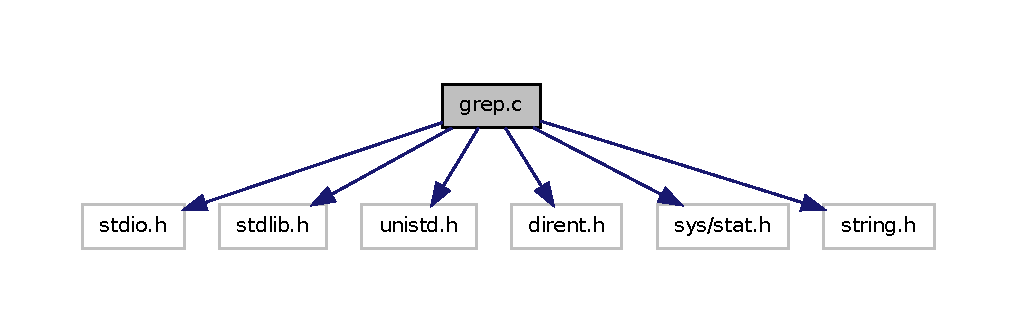
\includegraphics[width=400pt]{grep_8c__incl}
\end{center}
\end{figure}
\subsection*{Data Structures}
\begin{DoxyCompactItemize}
\item 
struct \hyperlink{structparameter}{parameter}
\begin{DoxyCompactList}\small\item\em Process parameter;. \item\end{DoxyCompactList}\end{DoxyCompactItemize}
\subsection*{Functions}
\begin{DoxyCompactItemize}
\item 
int \hyperlink{grep_8c_aabb59ed6fc07851912562b65b2094a10}{search\_\-ignore\_\-case} (const char $\ast$source, char $\ast$pattern)
\begin{DoxyCompactList}\small\item\em This function is used to define the search way-\/-\/-\/-\/$>$Ignore case;. \item\end{DoxyCompactList}\item 
int \hyperlink{grep_8c_a4fd56ab76f558b1679b08787ec370186}{search\_\-normal} (const char $\ast$source, char $\ast$pattern)
\begin{DoxyCompactList}\small\item\em This function is used to define the search way-\/-\/-\/-\/$>$Case sensitive. \item\end{DoxyCompactList}\item 
int \hyperlink{grep_8c_ac67113c7c9c189b5993995987ffd4be3}{search} (const char $\ast$source, char $\ast$pattern, char option, char choice)
\begin{DoxyCompactList}\small\item\em This function begins the search process;. \item\end{DoxyCompactList}\item 
int \hyperlink{grep_8c_a675badab75cb4a9b97fb5ac92669c4fb}{search\_\-file} (const char $\ast$source, char $\ast$pattern, char option)
\begin{DoxyCompactList}\small\item\em This function is used to search pattern in a file;. \item\end{DoxyCompactList}\item 
int \hyperlink{grep_8c_ad725f095d357ddd84e283d9d313f86e6}{process\_\-option} (int argc, char $\ast$argv\mbox{[}$\,$\mbox{]})
\begin{DoxyCompactList}\small\item\em Process the option information;. \item\end{DoxyCompactList}\item 
int \hyperlink{grep_8c_ac80385059968f2d1dd5fa9e1d054f43c}{read\_\-file} (const char $\ast$source, char $\ast$pattern, char option)
\begin{DoxyCompactList}\small\item\em This function is used to read file in different way;. \item\end{DoxyCompactList}\item 
int \hyperlink{grep_8c_af3b743a07d509e0e1cd535ceaaefb884}{search\_\-directory} (const char $\ast$source, char $\ast$pattern, char option)
\item 
int \hyperlink{grep_8c_a0ddf1224851353fc92bfbff6f499fa97}{main} (int argc, char $\ast$argv\mbox{[}$\,$\mbox{]})
\begin{DoxyCompactList}\small\item\em This is the main function;. \item\end{DoxyCompactList}\end{DoxyCompactItemize}
\subsection*{Variables}
\begin{DoxyCompactItemize}
\item 
struct \hyperlink{structparameter}{parameter} \hyperlink{grep_8c_a69277f024cd401bc6876e89a9d71d005}{param}
\begin{DoxyCompactList}\small\item\em Process parameter;. \item\end{DoxyCompactList}\end{DoxyCompactItemize}


\subsection{Detailed Description}
\begin{DoxyAuthor}{Author}
sunshine contact \href{mailto:mxdhlj@163.com}{\tt mxdhlj@163.com} 
\end{DoxyAuthor}
\begin{DoxyVersion}{Version}
0.00 
\end{DoxyVersion}
\begin{DoxyDate}{Date}
11-\/03-\/15 19:01:25 
\end{DoxyDate}


\subsection{Function Documentation}
\hypertarget{grep_8c_a0ddf1224851353fc92bfbff6f499fa97}{
\index{grep.c@{grep.c}!main@{main}}
\index{main@{main}!grep.c@{grep.c}}
\subsubsection[{main}]{\setlength{\rightskip}{0pt plus 5cm}int main (
\begin{DoxyParamCaption}
\item[{int}]{ argc, }
\item[{char $\ast$}]{ argv\mbox{[}$\,$\mbox{]}}
\end{DoxyParamCaption}
)}}
\label{grep_8c_a0ddf1224851353fc92bfbff6f499fa97}


This is the main function;. 


\begin{DoxyParams}{Parameters}
\item[{\em argc}]\item[{\em argv\mbox{[}$\,$\mbox{]}}]\end{DoxyParams}
\begin{DoxyReturn}{Returns}

\end{DoxyReturn}


Here is the call graph for this function:
\nopagebreak
\begin{figure}[H]
\begin{center}
\leavevmode
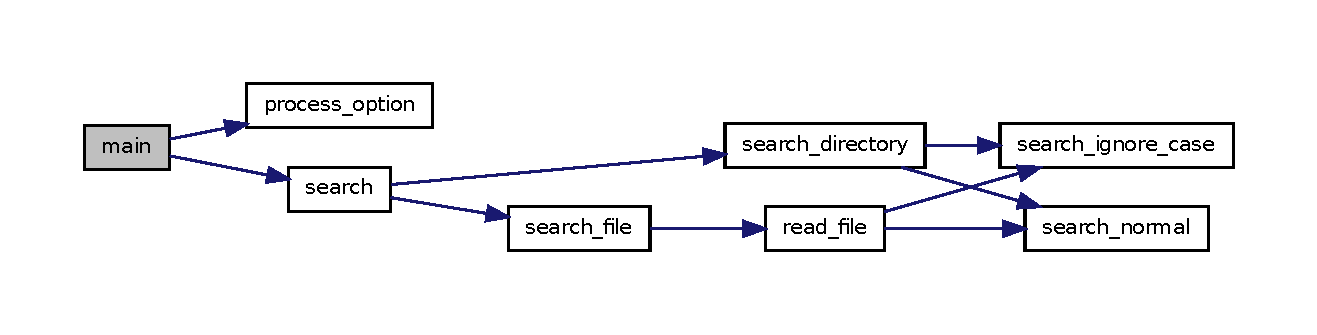
\includegraphics[width=400pt]{grep_8c_a0ddf1224851353fc92bfbff6f499fa97_cgraph}
\end{center}
\end{figure}


\hypertarget{grep_8c_ad725f095d357ddd84e283d9d313f86e6}{
\index{grep.c@{grep.c}!process\_\-option@{process\_\-option}}
\index{process\_\-option@{process\_\-option}!grep.c@{grep.c}}
\subsubsection[{process\_\-option}]{\setlength{\rightskip}{0pt plus 5cm}int process\_\-option (
\begin{DoxyParamCaption}
\item[{int}]{ argc, }
\item[{char $\ast$}]{ argv\mbox{[}$\,$\mbox{]}}
\end{DoxyParamCaption}
)}}
\label{grep_8c_ad725f095d357ddd84e283d9d313f86e6}


Process the option information;. 


\begin{DoxyParams}{Parameters}
\item[{\em argc}]\item[{\em argv\mbox{[}$\,$\mbox{]}}]\end{DoxyParams}
\begin{DoxyReturn}{Returns}

\end{DoxyReturn}


Here is the caller graph for this function:\nopagebreak
\begin{figure}[H]
\begin{center}
\leavevmode
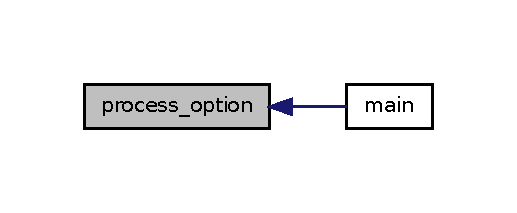
\includegraphics[width=248pt]{grep_8c_ad725f095d357ddd84e283d9d313f86e6_icgraph}
\end{center}
\end{figure}


\hypertarget{grep_8c_ac80385059968f2d1dd5fa9e1d054f43c}{
\index{grep.c@{grep.c}!read\_\-file@{read\_\-file}}
\index{read\_\-file@{read\_\-file}!grep.c@{grep.c}}
\subsubsection[{read\_\-file}]{\setlength{\rightskip}{0pt plus 5cm}int read\_\-file (
\begin{DoxyParamCaption}
\item[{const char $\ast$}]{ source, }
\item[{char $\ast$}]{ pattern, }
\item[{char}]{ option}
\end{DoxyParamCaption}
)}}
\label{grep_8c_ac80385059968f2d1dd5fa9e1d054f43c}


This function is used to read file in different way;. 


\begin{DoxyParams}{Parameters}
\item[{\em source}]\item[{\em pattern}]\item[{\em option}]\end{DoxyParams}
\begin{DoxyReturn}{Returns}

\end{DoxyReturn}


Here is the call graph for this function:\nopagebreak
\begin{figure}[H]
\begin{center}
\leavevmode
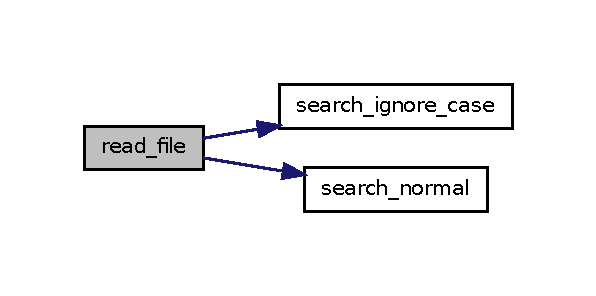
\includegraphics[width=286pt]{grep_8c_ac80385059968f2d1dd5fa9e1d054f43c_cgraph}
\end{center}
\end{figure}




Here is the caller graph for this function:\nopagebreak
\begin{figure}[H]
\begin{center}
\leavevmode
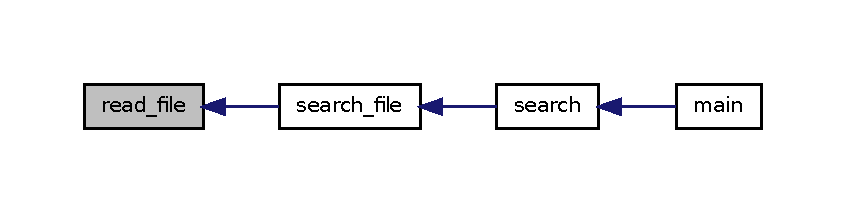
\includegraphics[width=400pt]{grep_8c_ac80385059968f2d1dd5fa9e1d054f43c_icgraph}
\end{center}
\end{figure}


\hypertarget{grep_8c_ac67113c7c9c189b5993995987ffd4be3}{
\index{grep.c@{grep.c}!search@{search}}
\index{search@{search}!grep.c@{grep.c}}
\subsubsection[{search}]{\setlength{\rightskip}{0pt plus 5cm}int search (
\begin{DoxyParamCaption}
\item[{const char $\ast$}]{ source, }
\item[{char $\ast$}]{ pattern, }
\item[{char}]{ option, }
\item[{char}]{ choice}
\end{DoxyParamCaption}
)}}
\label{grep_8c_ac67113c7c9c189b5993995987ffd4be3}


This function begins the search process;. 


\begin{DoxyParams}{Parameters}
\item[{\em source}]\item[{\em pattern}]\item[{\em option}]\item[{\em choice}]\end{DoxyParams}
\begin{DoxyReturn}{Returns}

\end{DoxyReturn}


Here is the call graph for this function:
\nopagebreak
\begin{figure}[H]
\begin{center}
\leavevmode
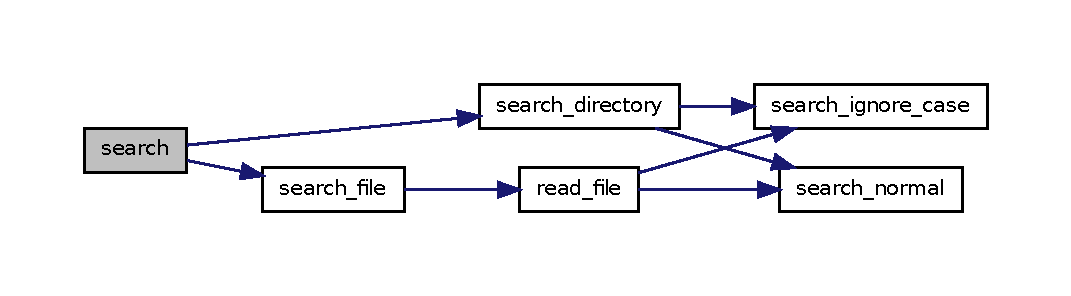
\includegraphics[width=400pt]{grep_8c_ac67113c7c9c189b5993995987ffd4be3_cgraph}
\end{center}
\end{figure}




Here is the caller graph for this function:\nopagebreak
\begin{figure}[H]
\begin{center}
\leavevmode
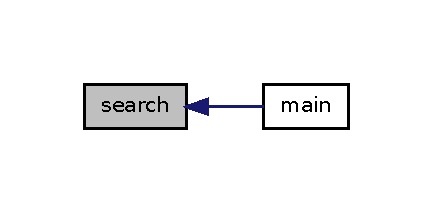
\includegraphics[width=208pt]{grep_8c_ac67113c7c9c189b5993995987ffd4be3_icgraph}
\end{center}
\end{figure}


\hypertarget{grep_8c_af3b743a07d509e0e1cd535ceaaefb884}{
\index{grep.c@{grep.c}!search\_\-directory@{search\_\-directory}}
\index{search\_\-directory@{search\_\-directory}!grep.c@{grep.c}}
\subsubsection[{search\_\-directory}]{\setlength{\rightskip}{0pt plus 5cm}int search\_\-directory (
\begin{DoxyParamCaption}
\item[{const char $\ast$}]{ source, }
\item[{char $\ast$}]{ pattern, }
\item[{char}]{ option}
\end{DoxyParamCaption}
)}}
\label{grep_8c_af3b743a07d509e0e1cd535ceaaefb884}


Here is the call graph for this function:
\nopagebreak
\begin{figure}[H]
\begin{center}
\leavevmode
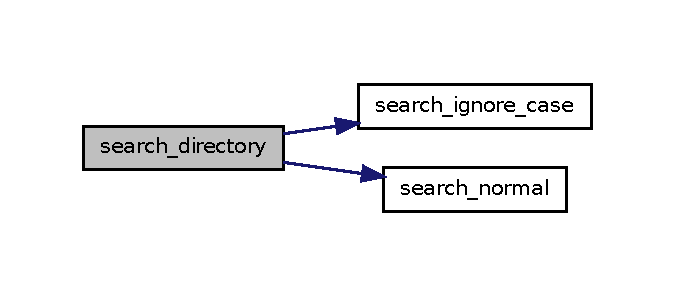
\includegraphics[width=324pt]{grep_8c_af3b743a07d509e0e1cd535ceaaefb884_cgraph}
\end{center}
\end{figure}




Here is the caller graph for this function:
\nopagebreak
\begin{figure}[H]
\begin{center}
\leavevmode
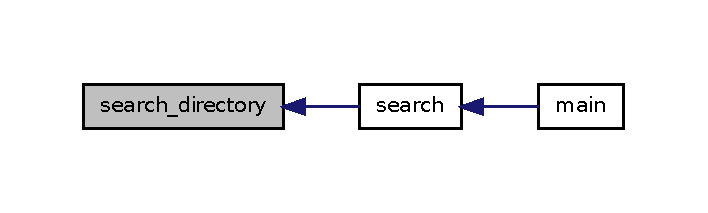
\includegraphics[width=340pt]{grep_8c_af3b743a07d509e0e1cd535ceaaefb884_icgraph}
\end{center}
\end{figure}


\hypertarget{grep_8c_a675badab75cb4a9b97fb5ac92669c4fb}{
\index{grep.c@{grep.c}!search\_\-file@{search\_\-file}}
\index{search\_\-file@{search\_\-file}!grep.c@{grep.c}}
\subsubsection[{search\_\-file}]{\setlength{\rightskip}{0pt plus 5cm}int search\_\-file (
\begin{DoxyParamCaption}
\item[{const char $\ast$}]{ source, }
\item[{char $\ast$}]{ pattern, }
\item[{char}]{ option}
\end{DoxyParamCaption}
)}}
\label{grep_8c_a675badab75cb4a9b97fb5ac92669c4fb}


This function is used to search pattern in a file;. 


\begin{DoxyParams}{Parameters}
\item[{\em source}]\item[{\em pattern}]\item[{\em option}]\end{DoxyParams}
\begin{DoxyReturn}{Returns}

\end{DoxyReturn}


Here is the call graph for this function:\nopagebreak
\begin{figure}[H]
\begin{center}
\leavevmode
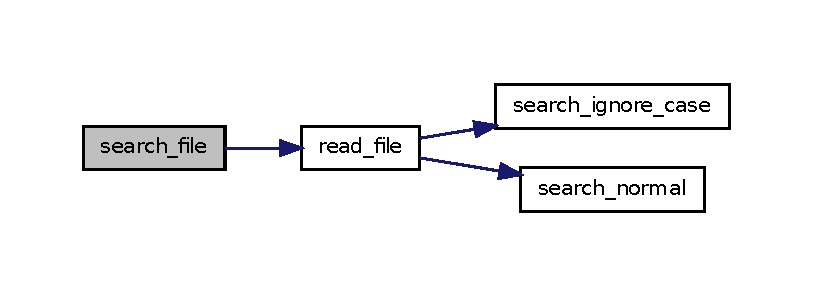
\includegraphics[width=390pt]{grep_8c_a675badab75cb4a9b97fb5ac92669c4fb_cgraph}
\end{center}
\end{figure}




Here is the caller graph for this function:\nopagebreak
\begin{figure}[H]
\begin{center}
\leavevmode
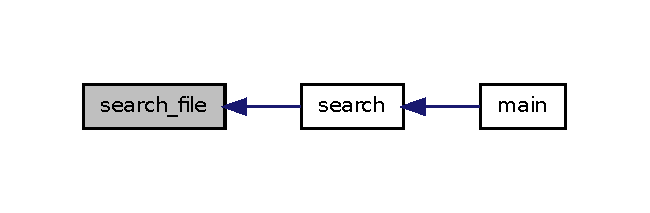
\includegraphics[width=312pt]{grep_8c_a675badab75cb4a9b97fb5ac92669c4fb_icgraph}
\end{center}
\end{figure}


\hypertarget{grep_8c_aabb59ed6fc07851912562b65b2094a10}{
\index{grep.c@{grep.c}!search\_\-ignore\_\-case@{search\_\-ignore\_\-case}}
\index{search\_\-ignore\_\-case@{search\_\-ignore\_\-case}!grep.c@{grep.c}}
\subsubsection[{search\_\-ignore\_\-case}]{\setlength{\rightskip}{0pt plus 5cm}int search\_\-ignore\_\-case (
\begin{DoxyParamCaption}
\item[{const char $\ast$}]{ source, }
\item[{char $\ast$}]{ pattern}
\end{DoxyParamCaption}
)}}
\label{grep_8c_aabb59ed6fc07851912562b65b2094a10}


This function is used to define the search way-\/-\/-\/-\/$>$Ignore case;. 


\begin{DoxyParams}{Parameters}
\item[{\em source}]\item[{\em pattern}]\end{DoxyParams}
\begin{DoxyReturn}{Returns}

\end{DoxyReturn}


Here is the caller graph for this function:
\nopagebreak
\begin{figure}[H]
\begin{center}
\leavevmode
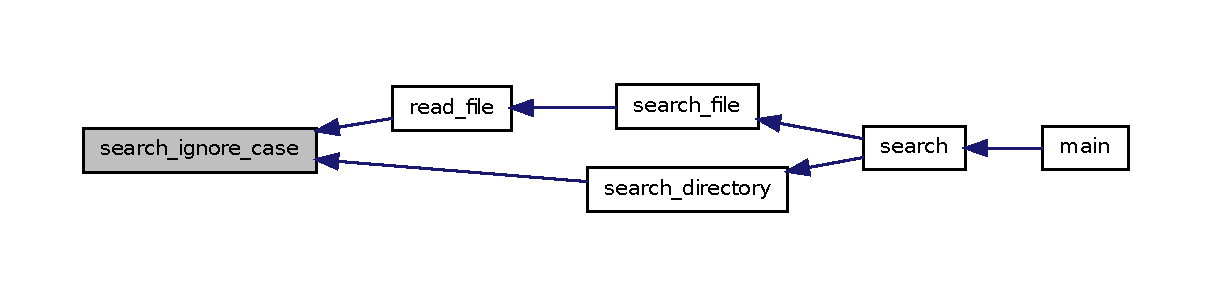
\includegraphics[width=400pt]{grep_8c_aabb59ed6fc07851912562b65b2094a10_icgraph}
\end{center}
\end{figure}


\hypertarget{grep_8c_a4fd56ab76f558b1679b08787ec370186}{
\index{grep.c@{grep.c}!search\_\-normal@{search\_\-normal}}
\index{search\_\-normal@{search\_\-normal}!grep.c@{grep.c}}
\subsubsection[{search\_\-normal}]{\setlength{\rightskip}{0pt plus 5cm}int search\_\-normal (
\begin{DoxyParamCaption}
\item[{const char $\ast$}]{ source, }
\item[{char $\ast$}]{ pattern}
\end{DoxyParamCaption}
)}}
\label{grep_8c_a4fd56ab76f558b1679b08787ec370186}


This function is used to define the search way-\/-\/-\/-\/$>$Case sensitive. 


\begin{DoxyParams}{Parameters}
\item[{\em source}]\item[{\em pattern}]\end{DoxyParams}
\begin{DoxyReturn}{Returns}

\end{DoxyReturn}


Here is the caller graph for this function:
\nopagebreak
\begin{figure}[H]
\begin{center}
\leavevmode
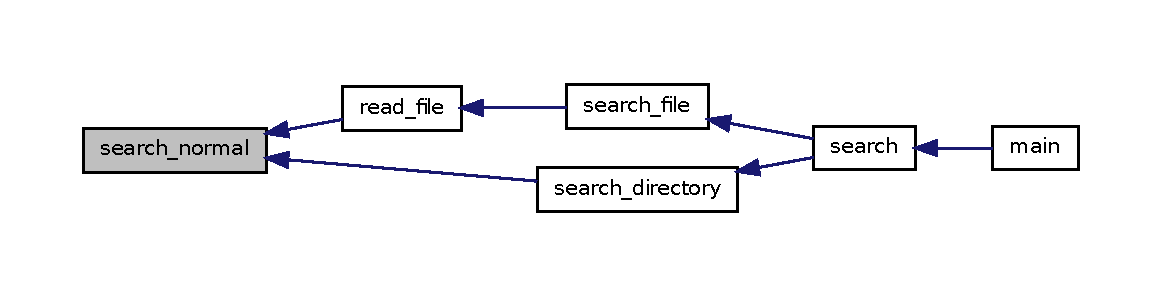
\includegraphics[width=400pt]{grep_8c_a4fd56ab76f558b1679b08787ec370186_icgraph}
\end{center}
\end{figure}




\subsection{Variable Documentation}
\hypertarget{grep_8c_a69277f024cd401bc6876e89a9d71d005}{
\index{grep.c@{grep.c}!param@{param}}
\index{param@{param}!grep.c@{grep.c}}
\subsubsection[{param}]{\setlength{\rightskip}{0pt plus 5cm}struct {\bf parameter} {\bf param}}}
\label{grep_8c_a69277f024cd401bc6876e89a9d71d005}


Process parameter;. 


\printindex
\end{document}
